\appendix

% \section{Extension of the Two-Rounds Algorithm}
% \label{chap1-sec:modified_two_rounds}
% aaa

\section{Effectiveness of empirical estimation in \alg{LocalRR$_\triangle$}}
\label{chap1-sec:RR_emp}
In Section~\ref{chap1-sub:non-interactive_triangles}, we presented \alg{LocalRR$_\triangle$}, which uses the empirical estimation method after the RR. 
Here we show the effectiveness of empirical estimation by comparing \alg{LocalRR$_\triangle$} with the RR without empirical estimation. 
% i.e., the randomized neighbor list in \cite{qin2017generating}. 
% This method was also used in \cite{Ye_ICDE20}. 
We also note that the RR has been applied to the adjacency matrix without empirical estimation in \cite{qin2017generating,Ye_ICDE20} for different purposes than counting triangles. 

As the RR without empirical estimation, we applied the RR to the lower triangular part of the adjacency matrix $\bmA$; i.e., we ran lines 1 to 6 in Algorithm~\ref{chap1-alg:subgraph-rr}. 
% This is the extended version of the randomized neighbor list \cite{qin2017generating}, as described in Section
Then we output the number of noisy triangles $m_3$. 
We denote this algorithm by \alg{RR w/o emp}. 
% Both \alg{LocalRR$_\triangle$} and \alg{RR w/o emp} provide $\epsilon$-edge LDP and $\epsilon$-entire edge LDP. 

\begin{figure}[t]
\centering
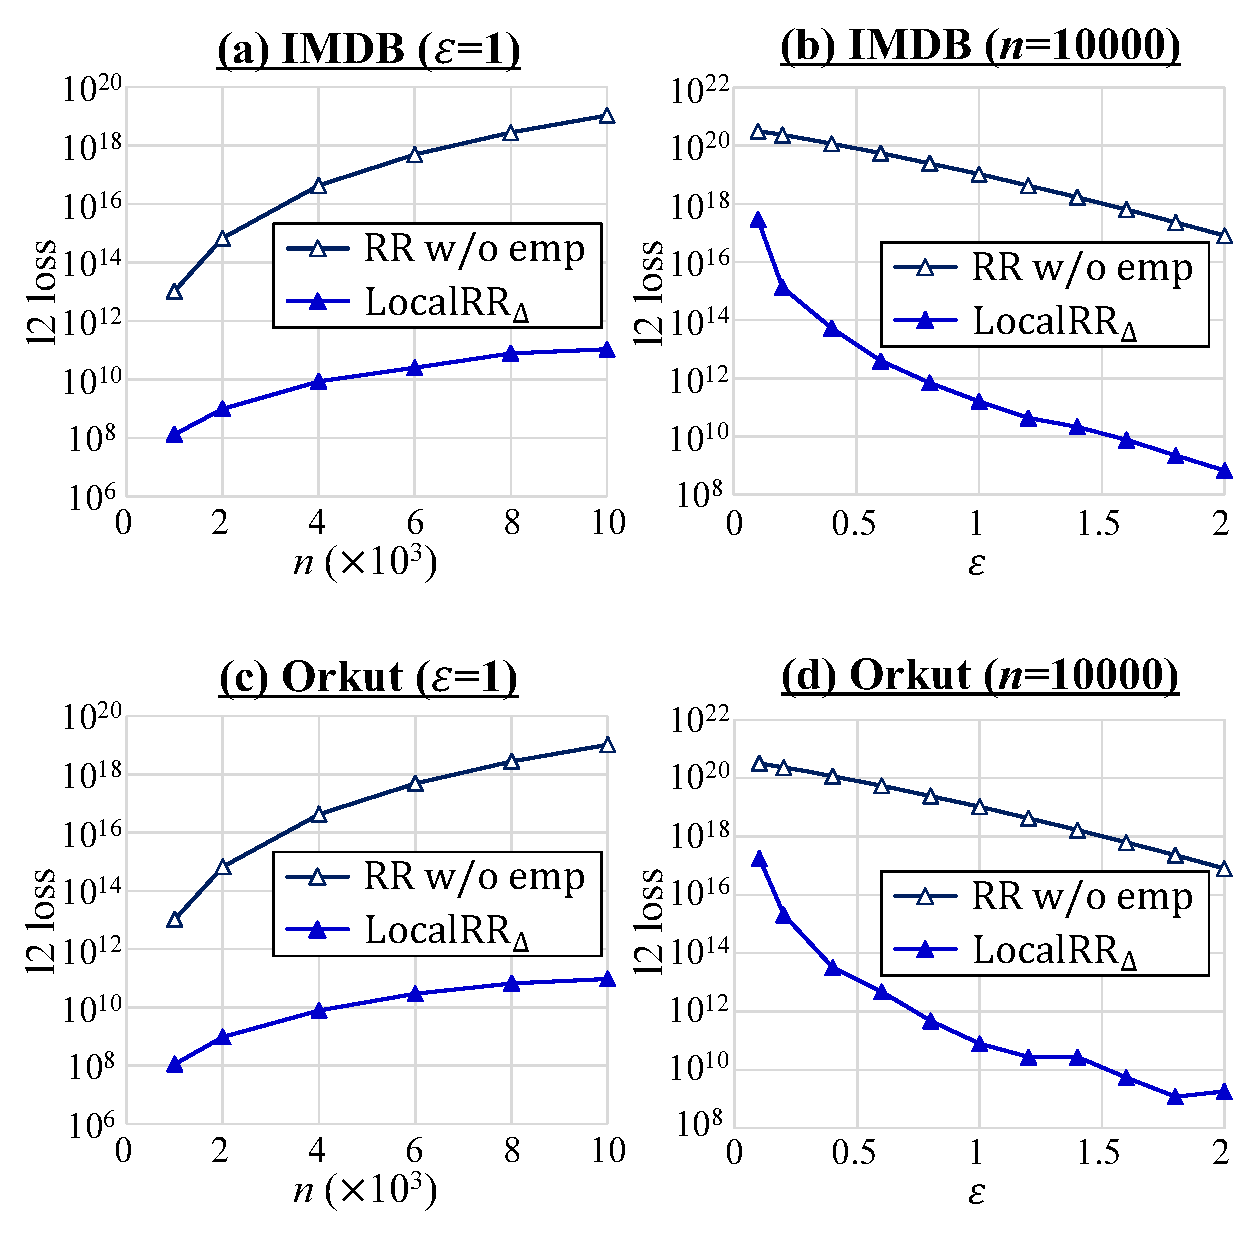
\includegraphics[width=0.99\linewidth]{fig/res5_RR_wo_emp.pdf}

\caption{$l_2$ loss of \alg{LocalRR$_\triangle$} and the RR without empirical estimation (\alg{RR w/o emp}).}
\label{chap1-fig:res5_RR_wo_emp}
\end{figure}

Figure~\ref{chap1-fig:res5_RR_wo_emp} shows the $l_2$ loss of \alg{LocalRR$_\triangle$} and \alg{RR w/o emp} when we changed $n$ from $1000$ to $10000$ or $\epsilon$ in edge LDP from $0.1$ to $2$. 
The experimental set-up is the same as Section~\ref{chap1-sub:setup}. 
Figure~\ref{chap1-fig:res5_RR_wo_emp} shows that \alg{LocalRR$_\triangle$} significantly outperforms \alg{RR w/o emp}, which means that the $l_2$ loss is significantly reduced by empirical estimation. 
As shown in Section~\ref{chap1-sec:experiments}, the $l_2$ loss of \alg{LocalRR$_\triangle$} is also significantly reduced by an additional round of interaction.

\section{Proof of Statements in Section~\ref{chap1-sec:algorithms}}
\label{chap1-sec:proof}
Here we prove the statements in Section~\ref{chap1-sec:algorithms}. 
Our proofs will repeatedly use the well-known bias-variance decomposition \cite{mlpp}, which we briefly explain below. 
We denote the variance of the random variable $X$ by $\mathbb{V}[X]$. 
If we are producing a private, randomized estimate $\hat{f}(G)$ of the graph function $f(G)$, then the expected $l_2$ loss can be written as: 
\begin{equation}\label{chap1-eq:bias-var}
  \E[l_2^2(\hat{f}(G),f(G))] = \left(\E[\hat{f}(G)] - f(G)\right)^2
  + \V[\hat{f}(G)].
\end{equation}
The first term is the bias, and the second term is the variance. 
If the estimate is unbiased (i.e., $\E[\hat{f}(G)] = f(G)$), then the expected $l_2$ loss is equal to the variance.

\subsection{Proof of Theorem~\ref{chap1-thm:k-stars_LDP}}
Let $\calR_i$ be \alg{LocalLap$_{k\star}$}. 
Let $d_i,d'_i \in \nnints$ be the number of ``1''s in two neighbor lists $\bma_i,\bma'_i \in \{0,1\}^n$ that differ in one bit. 
% Consider two neighbor lists $\bma_i,\bma'_i \in \{0,1\}^n$ that differ in one bit. 
% Let $d_i$ (resp.~$d'_i$) $\in \nnints$ be the number of ``1''s in $\bma_i$ (resp.~$\bma'_i$). 
Let $r_i = \binom{d_i}{k}$ and $r'_i = \binom{d'_i}{k}$. 
Below we consider two cases about $d_i$: when $d_i < \td_{max}$ and when $d_i \geq \td_{max}$.

\smallskip
\noindent{\textbf{Case 1: $d_i < \td_{max}$.}}~~In this case, both $\bma_i$ and $\bma'_i$ do not change after graph projection, as $d'_i \leq d_i + 1 \leq \td_{max}$. 
Then we obtain:
\begin{align*}
\Pr[\calR_i(\bma_i) = \hr_i] &= \exp\left(-\frac{\epsilon |\hr_i- r_i|}{\Delta}\right) \\
\Pr[\calR_i(\bma'_i) = \hr_i] &= \exp\left(-\frac{\epsilon |\hr_i- r'_i|}{\Delta}\right),
\end{align*}
where $\Delta = \binom{\td_{max}}{k-1}$. 
Therefore, 
% and hence 
\begin{align}
\frac{\Pr[\calR_i(\bma_i) = \hr_i]}{\Pr[\calR_i(\bma'_i) = \hr_i]} 
&= \exp\left( \frac{\epsilon |\hr_i- r'_i|}{\Delta} - \frac{\epsilon |\hr_i- r_i|}{\Delta}\right) \nonumber\\
&\leq  \exp\left( \frac{\epsilon |r'_i- r_i|}{\Delta} \right) \label{chap1-eq:Pr_R_i_a'_i_a_i}\\
& \hspace{4mm} (\text{by the triangle inequality}). \nonumber
\end{align}
If $d'_i = d_i + 1$, then $|r'_i- r_i|$ in (\ref{chap1-eq:Pr_R_i_a'_i_a_i}) can be written as follows:
\begin{align*}
|r'_i- r_i| 
= \binom{d_i+1}{k} - \binom{d_i}{k} 
= \binom{d_i}{k-1}
< \binom{\td_{max}}{k-1}
= \Delta, 
\end{align*}
Since we add $\Lap(\frac{\Delta}{\epsilon})$ to $r_i$, we obtain:
\begin{align}
\Pr[\calR_i(\bma_i) = \hr_i] \leq e^\epsilon \Pr[\calR_i(\bma'_i) = \hr_i]. 
\label{chap1-eq:R_i_a_i_hr_i}
\end{align}
If $d'_i = d_i - 1$, then $|r'_i- r_i| = \binom{d_i}{k} - \binom{d_i-1}{k} = \binom{d_i-1}{k-1} < \Delta$ and (\ref{chap1-eq:R_i_a_i_hr_i}) holds. 
Therefore, \alg{LocalLap$_{k\star}$} provides $\epsilon$-edge LDP. 

\smallskip
\noindent{\textbf{Case 2: $d_i \geq \td_{max}$.}}~~Assume 
% Second, we consider the case where $d_i \geq \td_{max}$. 
that $d'_i = d_i + 1$. 
In this case, $d'_i > \td_{max}$. 
Therefore, $d'_i$ becomes $\td_{max}$ after graph projection. 
In addition, 
% If $d_i > \td_{max}$, then 
$d_i$ also becomes $\td_{max}$ after graph projection. 
Therefore, we obtain 
$d_i = d'_i = \td_{max}$ after graph projection. 
Thus 
% and $r_i = r'_i = \binom{\td_{max}}{k}$. 
% Therefore, 
$\Pr[\calR_i(\bma_i) = \hr_i] = \Pr[\calR_i(\bma'_i) = \hr_i]$. 

Assume that $d'_i = d_i - 1$. 
If $d_i > \td_{max}$, then $d_i = d'_i = \td_{max}$ after graph projection. 
Thus $\Pr[\calR_i(\bma_i) = \hr_i] = \Pr[\calR_i(\bma'_i) = \hr_i]$. 
If $d_i = \td_{max}$, then (\ref{chap1-eq:R_i_a_i_hr_i}) holds. 
Therefore, \alg{LocalLap$_{k\star}$} provides $\epsilon$-edge LDP. \qed

\subsection{Proof of Theorem~\ref{chap1-thm:k-stars}}
Assuming the maximum degree $d_{max}$ of $G$ is at most $\td_{max}$, the only
randomness in the algorithm will be the Laplace noise since graph projection
will not occur.
Since the Laplacian noise $\Lap(\frac{\Delta}{\epsilon})$ has mean $0$, the estimate $\hf_{k\star}(G, \epsilon, \td_{max})$ is unbiased. 
Then by the bias-variance decomposition \cite{mlpp}, 
the expected $l_2$ loss 
$\mathbb{E}[l_2^2(\hf_{k\star}(G, \epsilon, \td_{max}),\allowbreak f_{k\star}(G))]$ is equal to the variance of $\hf_{k\star}(G, \epsilon, \td_{max})$. 
% We denote the variance of the random variable $X$ by $\mathbb{V}[X]$. 
The variance of $\hf_{k\star}(G, \epsilon, \td_{max})$ can be written as follows:
\begin{align*}
    \mathbb{V}[\hf_{k\star}(G, \epsilon, \td_{max})] 
    &= \mathbb{V}\left[ \sum_{i=1}^n \Lap\left( \frac{\Delta}{\epsilon} \right) \right] \\
    &= \frac{n \Delta^2}{\epsilon^2}.
\end{align*}
% Note that $\tilde{m}_3$ and $\tilde{m}_0$ are not dependent. 
Since $\Delta = \binom{\td_{max}}{k-1} = O(\td_{max}^{k-1})$, we obtain:
\begin{align*}
    \mathbb{E}[l_2^2(\hf_{k\star}(G, \epsilon, \td_{max}), f_{k\star}(G))] 
    &= \mathbb{V}[\hf_{k\star}(G, \epsilon, \td_{max})] \\
    &= O\left(\frac{n \td_{max}^{2k-2}}{\epsilon^2}\right).
\end{align*}
\qed

\subsection{Proof of Proposition~\ref{chap1-prop:triangle_emp}}
Let $\mu = e^\epsilon$ and $\bmQ \in [0,1]^{4 \times 4}$ be a $4 \times 4$ matrix such that:
\begin{align}
  \bmQ = \frac{1}{(\mu+1)^3} \left(
    \begin{array}{cccc}
      \mu^3 & 3\mu^2 & 3\mu & 1 \\
      \mu^2 & \mu^3+2\mu & 2\mu^2+1 & \mu \\
      \mu & 2\mu^2+1 & \mu^3+2\mu & \mu^2 \\
      1 & 3\mu & 3\mu^2 & \mu^3
    \end{array}
  \right).
  \label{chap1-eq:Q_1}
\end{align}
Let $c_3, c_2, c_1, c_0 \in \nnints$ be respectively the number of triangles, 2-edges, 1-edge, and no-edges in $G$. 
Then we obtain:
\begin{align}
(\mathbb{E}[m_3], \mathbb{E}[m_2], \mathbb{E}[m_1],
\mathbb{E}[m_0]) = (c_3, c_2, c_1, c_0) \bmQ.
\label{chap1-eq:bmQ}
\end{align}
In other words, $\bmQ$ is a transition matrix from a type of subgraph (i.e., triangle, 2-edges, 1-edge, or no-edge) in $G$ to a type of subgraph in $G'$. 

Let $\hat{c}_3, \hat{c}_2, \hat{c}_1, \hat{c}_0 \in \reals$ be the empirical estimate of $(c_3, c_2, c_1, c_0)$. 
By (\ref{chap1-eq:bmQ}), they can be written as follows:
\begin{align}
(\hat{c}_3, \hat{c}_2, \hat{c}_1, \hat{c}_0) = (m_3, m_2, m_1, m_0) \bmQ^{-1}.
\label{chap1-eq:hc3_hc2_hc1_hc0}
\end{align}
Let $\bmQ_{i,j}^{-1}$ be the ($i,j$)-th element of $\bmQ^{-1}$. 
By using Cramer's rule, we obtain: 
\begin{align}
\bmQ_{1,1}^{-1} &= \textstyle{\frac{\mu^3}{(\mu-1)^3}},~ \bmQ_{2,1}^{-1} =  \textstyle{-\frac{\mu^2}{(\mu-1)^3}}, \label{chap1-eq:bmQ11_bmQ21}\\
\bmQ_{3,1}^{-1} &= \textstyle{\frac{\mu}{(\mu-1)^3}},~ \bmQ_{4,1}^{-1} = \textstyle{-\frac{1}{(\mu-1)^3}}.
\label{chap1-eq:bmQ31_bmQ41}
\end{align}
By (\ref{chap1-eq:hc3_hc2_hc1_hc0}), (\ref{chap1-eq:bmQ11_bmQ21}), and (\ref{chap1-eq:bmQ31_bmQ41}), we obtain:
\begin{align*}
\textstyle{\hat{c}_3 = \frac{\mu^3}{(\mu-1)^3} m_3 - \frac{\mu^2}{(\mu-1)^3} m_2 + \frac{\mu}{(\mu-1)^3} m_1 - \frac{1}{(\mu-1)^3} m_0.}
\end{align*}
Since the empirical estimate is unbiased \cite{Kairouz_ICML16,Wang_USENIX17}, we obtain (\ref{chap1-eq:triangle_emp}) in Proposition~\ref{chap1-prop:triangle_emp}. \qed

\subsection{Proof of Theorem~\ref{chap1-thm:subgraph-rr_LDP}}
Since \alg{LocalRR$_\triangle$} applies the RR to the lower triangular part of the adjacency matrix $\bmA$, it provides $\epsilon$-edge LDP for $(R_1, \ldots, R_n)$. 
Lines 5 to 8 in Algorithm~\ref{chap1-alg:subgraph-rr} are post-processing of $(R_1, \ldots, R_n)$. 
Thus, by the immunity to post-processing \cite{DP}, \alg{LocalRR$_\triangle$} provides $\epsilon$-edge LDP for the output $\frac{1}{(\mu-1)^3}(\mu^3 m_3 -\mu^2 m_2 + \mu m_1 - m_0)$. 

In addition, the existence of edge $(v_i,v_j) \in E$ $(i>j)$ affects only one element $a_{i,j}$ in the lower triangular part of $\bmA$. 
Therefore, \alg{LocalRR$_\triangle$} provides $\epsilon$-entire edge LDP.

\subsection{Proof of Theorem~\ref{chap1-thm:subgraph-rr}}
\label{chap1-sub:proof_thm:subgraph-rr}
By Proposition~\ref{chap1-prop:triangle_emp}, the estimate $\hf_{\triangle}(G, \epsilon)$ by \alg{LocalRR$_\triangle$} is unbiased. 
Then by the bias-variance decomposition \cite{mlpp}, 
the expected $l_2$ loss $\mathbb{E}[l_2^2(\hf_{\triangle}(G, \epsilon), f_\triangle(G))]$ is equal to the variance of $\hf_{\triangle}(G, \epsilon)$. 
% We denote the variance of the random variable $X$ by $\mathbb{V}[X]$. 
Let 
$a_3 = \frac{\mu^3}{(\mu-1)^3}$, 
$a_2 = - \frac{\mu^2}{(\mu-1)^3}$, 
$a_1 = \frac{\mu}{(\mu-1)^3}$, and 
$a_0 = - \frac{1}{(\mu-1)^3}$. 
Then the variance of $\hf_{\triangle}(G, \epsilon)$ can be written as follows:
\begin{align}
    \V[\hf_{\triangle}(G, \epsilon)] 
    &= \V[a_3 m_3 + a_2 m_2 + a_1 m_1 + a_0 m_0] \nonumber\\
    &= a_3^2 \V[m_3] + a_2^2 \V_{RR}[m_2] + a_1^2 \V[m_1] + a_0^2 \V[m_0] \nonumber\\
    &\hspace{3.5mm} + \sum_{i=0}^3 \sum_{j=0, j \ne i}^3 2a_i a_j \text{cov}(m_i, m_j),
    \label{chap1-eq:V_a3m3_a2m2_a1m1_a0m0}
\end{align}
where $\text{cov}(m_i, m_j)$ represents the covariance of $m_i$ and $m_j$. 
The covariance $\text{cov}(m_i, m_j)$ can be written as follows:
\begin{align}
    \text{cov}(m_i, m_j)
    &\leq \sqrt{\V[m_i] \V[m_j]} \nonumber\\
    &\hspace{4.2mm} (\text{by Cauchy-Schwarz inequality}) \nonumber\\
    &\leq  \max\{ \V[m_i], \V[m_j]\} \nonumber\\
    &\leq \V[m_i] + \V[m_j].
    \label{chap1-eq:cov_mi_mj}
\end{align}
By (\ref{chap1-eq:V_a3m3_a2m2_a1m1_a0m0}) and (\ref{chap1-eq:cov_mi_mj}), we obtain:
\begin{align}
    &\V[\hf_{\triangle}(G, \epsilon)] \nonumber\\
    &\leq (a_3^2 + 4a_3(a_2 + a_1 + a_0)) \V[m_3] \nonumber\\
    & \hspace{4.5mm} + (a_2^2 + 4a_2(a_3 + a_1 + a_0)) \V[m_2] \nonumber\\
    & \hspace{4.5mm} + (a_1^2 + 4a_1(a_3 + a_2 + a_0)) \V[m_1] \nonumber\\
    & \hspace{4.5mm} + (a_0^2 + 4a_0(a_3 + a_2 + a_1)) \V[m_0] \nonumber\\
    &= O\left( \frac{e^{6\epsilon}}{(e^\epsilon-1)^6} (\V[m_3] + \V[m_2] + \V[m_1] + \V[m_0]) \right).
    % &\leq O\left(\frac{e^{6\epsilon}}{(e^\epsilon-1)^6} \V[m_3] + \frac{e^{5\epsilon}}{(e^\epsilon-1)^6}\V[m_2]
    % \right. \nonumber\\
    % & \hspace{10mm} \left. + \frac{e^{4\epsilon}}{(e^\epsilon-1)^6}\V[m_1] + \frac{e^{3\epsilon}}{(e^\epsilon-1)^6}\V[m_0]\right).
    \label{chap1-V_RR_m_3}
\end{align}

Below we calculate $\V[m_3]$, $\V[m_2]$, $\V[m_1]$, and $\V[m_0]$ by assuming the Erd\"{o}s-R\'{e}nyi model $\bmG(n, \alpha)$ for $G$:

\begin{lemma}\label{chap1-lem:erdos-renyi-variance}
  Let $G \sim \textbf{G}(n,\alpha)$. 
  %with $\alpha < \frac{1}{2}$. 
  Let $p = \frac{1}{e^\epsilon+1}$ and 
  $\beta = \alpha(1-p) + (1-\alpha)p$. 
  Then $\V[m_3] = O(\beta^5 n^4 + \beta^3
  n^3)$, $\V[m_2] = O(\beta^3 n^4 + \beta^2 n^3)$, and 
  $\V[m_1] = \V[m_0] = O(\beta n^4)$.
\end{lemma}
% We prove Lemma~\ref{chap1-lem:erdos-renyi-variance} at the end of Appendix~\ref{chap1-sub:proof_thm:subgraph-rr}. 
Before going into the proof of Lemma~\ref{chap1-lem:erdos-renyi-variance}, we prove Theorem~\ref{chap1-thm:subgraph-rr} using Lemma~\ref{chap1-lem:erdos-renyi-variance}. 
By (\ref{chap1-V_RR_m_3}) and Lemma~\ref{chap1-lem:erdos-renyi-variance}, we obtain: 
\begin{align*}
\V[\hf_{\triangle}(G, \epsilon)] = O\left( \frac{e^{6\epsilon}}{(e^\epsilon-1)^6} \beta n^4 \right),
\end{align*}
which proves Theorem~\ref{chap1-thm:subgraph-rr}. \qed

We now prove Lemma~\ref{chap1-lem:erdos-renyi-variance}:

\begin{proof}[Proof of Lemma~\ref{chap1-lem:erdos-renyi-variance}]
Fist we show the variance of $m_3$ and $m_0$. 
Then we show the variance of $m_2$ and $m_1$.

\smallskip
\noindent{\textbf{Variance of $m_3$ and $m_0$.}}~~Since each edge in the original graph $G$ is independently generated with probability $\alpha \in [0,1]$, each edge in the noisy graph $G'$ is independently generated with probability $\beta = \alpha (1-p) + (1 - \alpha) p \in [0,1]$, where $p=\frac{1}{e^\epsilon+1}$. 
Thus $m_3$ is the number of triangles in graph $G' \sim \textbf{G}(n,\beta)$.

For $i,j,k \in [n]$, let $y_{i,j,k} \in \{0,1\}$ be a variable that takes $1$ if and only if 
$(v_i, v_j, v_k)$ forms a triangle. 
Then $\mathbb{E}[m_3^2]$ can be written as follows:
\begin{align}
  \mathbb{E}[m_3^2] = \sum_{i<j<k} ~ \sum_{i'<j'<k'}
  \mathbb{E}[y_{i,j,k} y_{i',j',k'}] 
  \label{chap1-eq:E_RR_tm3}
\end{align}
$\mathbb{E}[y_{i,j,k} y_{i',j',k'}]$ in (\ref{chap1-eq:E_RR_tm3}) is the probability that both $(v_i,v_j,v_k)$ and $(v_{i'},v_{j'},v_{k'})$ form a triangle. 
This event can be divided into the following four types:
\begin{enumerate}
\item $(i,j,k)=(i',j',k')$. There are $\binom{n}{3}$ such terms in (\ref{chap1-eq:E_RR_tm3}). 
For each term, $\mathbb{E}[y_{i,j,k} y_{i',j',k'}] = \beta^3$.
\item $(i,j,k)$ and $(i',j',k')$ have two elements in common. 
There are $\binom{n}{2} (n-2) (n-3) = 12\binom{n}{4}$ such terms in (\ref{chap1-eq:E_RR_tm3}). 
For each term, $\mathbb{E}[y_{i,j,k} y_{i',j',k'}] = \beta^5$. 
\item $(i,j,k)$ and $(i',j',k')$ have one element in common. 
There are $n \binom{n-1}{2} \binom{n-3}{2} = 30\binom{n}{5}$ such terms in (\ref{chap1-eq:E_RR_tm3}). 
For each term, $\mathbb{E}[y_{i,j,k} y_{i',j',k'}] = \beta^6$. 
\item $(i,j,k)$ and $(i',j',k')$ have no common elements. 
There are $\binom{n}{3} \binom{n-3}{3} = 20\binom{n}{6}$ such terms in in (\ref{chap1-eq:E_RR_tm3}). 
For each term, $\mathbb{E}[y_{i,j,k} y_{i',j',k'}] = \beta^6$. 
\end{enumerate}
Moreover, $\mathbb{E}[m_3]^2 = \binom{n}{3}^2 \beta^6$. 
Therefore, the variance of $m_3$ can be written as follows:
\begin{align*}
    \V[m_3] 
    &= \textstyle{\binom{n}{3} \beta^3 + 12\binom{n}{4} \beta^5 + 30\binom{n}{5} \beta^6 + 20\binom{n}{6} \beta^6 - \binom{n}{3}^2 \beta^6} \\
    &= \textstyle{\binom{n}{3} \beta^3 (1-\beta^3) + 12\binom{n}{4}\beta^5(1-\beta)} \\
    &= O(\beta^5 n^4 + \beta^3 n^3).
\end{align*}

By changing $\beta$ to $1-\beta$ and counting triangles, we get a random variable with the same distribution as $m_0$. Thus,
\begin{align*}
  \V[m_0] 
  &= \textstyle{\binom{n}{3} (1-\beta)^3(1-(1-\beta)^3) + 12\binom{n}{4} (1-\beta)^5\beta}
  \\
  &= O(\beta n^4).
\end{align*}
\smallskip
\noindent{\textbf{Variance of $m_2$ and $m_1$.}}~~For $i,j,k \in [n]$, let $z_{i,j,k} \in \{0,1\}$ be a variable that takes $1$ if and only if 
$(v_i, v_j, v_k)$ forms $2$-edges (i.e., exactly one edge is missing in the three nodes). 
Then $\mathbb{E}[m_2^2]$ can be written as follows:
\begin{align}
  \mathbb{E}[m_2^2] = \sum_{i<j<k} \sum_{i'<j'<k'}
  \mathbb{E}[z_{i,j,k} z_{i',j',k'}] 
  \label{chap1-eq:E_RR_tm2}
\end{align}
$\mathbb{E}[z_{i,j,k} z_{i',j',k'}]$ in (\ref{chap1-eq:E_RR_tm2}) is the probability that both $(v_i,v_j,v_k)$ and $(v_{i'},v_{j'},v_{k'})$ form $2$-edges. 
This event can be divided into the following four types:
\begin{enumerate}
	\item $(i,j,k)=(i',j',k')$. There are $\binom{n}{3}$ such terms in (\ref{chap1-eq:E_RR_tm2}). 
    For each term, $\mathbb{E}[z_{i,j,k} z_{i',j',k'}]=3\beta^2(1-\beta)$. 
	\item $(i,j,k)$ and $(i',j',k')$ have two elements in common. 
	There are $\binom{n}{2}(n-2)(n-3) = 12 \binom{n}{4}$ such terms in (\ref{chap1-eq:E_RR_tm2}). 
	For example, consider a term in which $i=i'=1$, $j=j'=2$, $k=3$, and $k'=4$. 
	Both $(v_1,v_2,v_3)$ and $(v_1,v_2,v_4)$ form 2-edges if:\\
	(a) $(v_1,v_2), (v_1,v_3), (v_1,v_4) \in E'$, $(v_2,v_3), (v_2,v_4) \notin E'$, \\
	(b) $(v_1,v_2), (v_1,v_3), (v_2,v_4) \in E'$, $(v_2,v_3), (v_1,v_4) \notin E'$, \\
	(c) $(v_1,v_2), (v_2,v_3), (v_1,v_4) \in E'$, $(v_1,v_3), (v_2,v_4) \notin E'$, \\
	(d) $(v_1,v_2), (v_2,v_3), (v_2,v_4) \in E'$, $(v_1,v_3), (v_1,v_4) \notin E'$, or \\
	(e) $(v_1,v_3), (v_1,v_4), (v_2,v_3), (v_2,v_4) \in E'$, $(v_1,v_2) \notin E'$. \\
    Thus, $\mathbb{E}[z_{i,j,k} z_{i',j',k'}]=4\beta^3(1-\beta)^2 + \beta^4(1-\beta)$ for this term. 
    Similarly, $\mathbb{E}[z_{i,j,k} z_{i',j',k'}]=4\beta^3(1-\beta)^2 + \beta^4(1-\beta)$ for the other terms.
	\item $(i,j,k)$ and $(i',j',k')$ have one element in common. 
	There are $n \binom{n-1}{2} \binom{n-3}{2} = 30\binom{n}{5}$ such terms in (\ref{chap1-eq:E_RR_tm2}).  For each term, $\mathbb{E}[z_{i,j,k}z_{i',j',k'}]=(3\beta^2(1-\beta))^2 = 9\beta^4(1-\beta)^2$. 
	\item $(i,j,k)$ and $(i',j',k')$ have no common elements. 
	There are $\binom{n}{3}\binom{n-3}{3} = 20\binom{n}{6}$ such terms in (\ref{chap1-eq:E_RR_tm2}). 
	For each term, $\mathbb{E}[z_{i,j,k}z_{i',j',k'}]=(3\beta^2(1-\beta))^2 = 9\beta^4(1-\beta)^2$. 
\end{enumerate}
Moreover, $\mathbb{E}[m_2]^2 = (3\binom{n}{3}\beta^2(1-\beta))^2 = 9\binom{n}{3}^2\beta^4(1-\beta)^2$. 
Therefore, the variance of $m_2$ can be written as follows:
\begin{align*}
  \mathbb{V}[m_2] 
  &= \mathbb{E}[m_2^2] - \mathbb{E}[m_2]^2 \nonumber\\
  &= \textstyle{3\binom{n}{3}\beta^2(1-\beta) + 12\binom{n}{4}\left(4\beta^3(1-\beta)^2 + \beta^4(1-\beta)\right)} \nonumber\\
  &\hspace{3.5mm} \textstyle{+ 270\binom{n}{5}\beta^4(1-\beta)^2 + 180\binom{n}{6}\beta^4(1-\beta)^2} \nonumber\\
  &\hspace{3.5mm} \textstyle{- 9\binom{n}{3}^2\beta^4(1-\beta)^2.}
\end{align*}
By simple calculations,
\begin{align*}
\textstyle{270\binom{n}{5} + 180\binom{n}{6} - 9\binom{n}{3}^2 = -108\binom{n}{4}-9\binom{n}{3}.}
\end{align*}
Thus we obtain:
\begin{align*}
\mathbb{V}[m_2] 
&= \textstyle{3\binom{n}{3}\beta^2(1-\beta)\left(1 - 3\beta^2(1-\beta)\right)} \nonumber\\
%&\hspace{3.5mm} \textstyle{+ 12\binom{n}{4}\left(4\beta^3(1-\beta)^2 + \beta^4(1-\beta) - 9\beta(1-\beta) \right)} \\
&\hspace{3.5mm} \textstyle{+ 12\binom{n}{4} \beta^3(1-\beta) \left(4(1-\beta) + \beta - 9\beta(1-\beta) \right)} \\
&= O(\beta^3 n^4 + \beta^2n^3).
\end{align*}
Similarly, the variance of $m_1$ can be written as follows:
\begin{align*}
\mathbb{V}[m_1] 
&= \textstyle{3\binom{n}{3}\beta(1-\beta)^2\left(1 - 3\beta(1-\beta)^2\right)} \nonumber\\
&\hspace{3.5mm} \textstyle{+ 12\binom{n}{4} \beta(1-\beta)^3 \left(4\beta +
(1-\beta) - 9\beta(1-\beta) \right)} \\
&= O(\beta n^4).
\end{align*}
\end{proof}

\subsection{Proof of Proposition~\ref{chap1-prop:triangle_emp_2rounds}}
Let $t_* = \sum_{i=1}^n t_i$ and $s_* = \sum_{i=1}^n s_i$. 
Let $s_*^{\wedge}$ be the number of triplets $(v_i,v_j,v_k)$ such that $j<k<i$, $a_{i,j} = a_{i,k} = 1$, and $a_{j,k} = 0$. 
Let $s_*^{\triangle}$ be the number of triplets $(v_i,v_j,v_k)$ such that $j<k<i$, $a_{i,j} = a_{i,k} = a_{j,k} =1$. 
Note that 
$s_* = s_*^{\wedge} + s_*^{\triangle}$ and 
$s_*^{\triangle} = f_\triangle(G)$. 

Consider a triangle $(v_i,v_j,v_k) \in G$. 
This triangle is counted $1-p_1$ ($= \frac{e^{\epsilon_1}}{e^{\epsilon_1}+1}$) times in expectation in $t_*$. 
Consider $2$-edges $(v_i,v_j,v_k) \in G$ (i.e., exactly one edge is missing in the three nodes). 
This is counted $p_1$ ($= \frac{1}{e^{\epsilon_1}+1}$) times in expectation in $t_*$.  
No other events can change $t_*$. 
% Thus, with respect to the randomness in the graph $G'$,
Therefore, we obtain:
\begin{align*}
\mathbb{E}[t_*] = (1-p_1) s_*^{\triangle} + p_1 s_*^{\wedge}. 
\end{align*}
By $s_* = s_*^{\wedge} + s_*^{\triangle}$ and 
$s_*^{\triangle} = f_\triangle(G)$, we obtain:
\begin{align*}
\mathbb{E}\left[\sum_{i=1}^n w_i \right] 
&= \mathbb{E}\left[\sum_{i=1}^n (t_i - p_1 s_i) \right] \\
&= \mathbb{E}[t_* - p_1 s_*] \\
&= \mathbb{E}[t_*] - p_1 \mathbb{E}[s_*^{\wedge} + s_*^{\triangle}] \\
&= (1-p_1) s_*^{\triangle} + p_1 s_*^{\wedge} - p_1 (s_*^{\wedge} + s_*^{\triangle}) \\
&= (1 - 2 p_1) f_\triangle(G),
\end{align*}
hence 
\begin{align*}
\textstyle{\mathbb{E}\left[ \frac{1}{1-2p_1} \sum_{i=1}^n w_i \right] = f_\triangle(G).}
\end{align*}
\qed

\subsection{Proof of Theorem~\ref{chap1-thm:local2rounds_LDP}}
Let $\calR_i$ be \alg{Local2Rounds$_{\triangle}$}. 
Consider two neighbor lists $\bma_i,\bma'_i \in \{0,1\}^n$ that differ in one bit. 
Let $d_i$ (resp.~$d'_i$) $\in \nnints$ be the number of ``1''s in $\bma_i$ (resp.~$\bma'_i$). 
Let $\bbma_i$ (resp.~$\bbma'_i$) $\in \{0,1\}^n$ be neighbor lists obtained by setting all of the $i$-th to the $n$-th elements in $\bma_i$ (resp.~$\bma'_i$) to $0$. 
Let $\bd_i$ (resp.~$\bd'_i$) $\in \nnints$ be the number of ``1''s in $\bbma_i$ (resp.~$\bbma'_i$). 
% from the first to the $(i-1)$-th elements in $\bma_i$ (resp.~$\bma'_i$). 
For example, if $n=6$, $\bma_4=(1,0,1,0,1,1)$, and $\bma'_4=(1,1,1,0,1,1)$, then 
$d_4=4$, $d'_4=5$, $\bbma_4=(1,0,1,0,0,0)$, $\bbma'_4=(1,1,1,0,0,0)$, $\bd_4=2$, and $\bd'_4=3$. 

Furthermore, 
let $t_i$ (resp.~$t'_i$) $\in \nnints$ be the number of triplets $(v_i, v_j, v_k)$ such that $j < k < i$, $(v_i,v_j) \in E$, $(v_i,v_k) \in E$, and $(v_j,v_k) \in E'$ in $\bma_i$ (resp.~$\bma'_i$). 
Let $s_i$ (resp.~$s'_i$) $\in \nnints$ be the number of triplets $(v_i, v_j, v_k)$ such that $j < k < i$, $(v_i,v_j) \in E$, and $(v_i,v_k) \in E$ in $\bma_i$ (resp.~$\bma'_i$). 
Let $w_i = t_i - p_1 s_i$ and $w'_i = t'_i - p_1 s'_i$. 
Below we consider two cases about $d_i$: when $d_i < \td_{max}$ and when $d_i \geq \td_{max}$. 

\smallskip
\noindent{\textbf{Case 1: $d_i < \td_{max}$.}}~~Assume that $d'_i = d_i + 1$. 
In this case, we have either $\bbma'_i = \bbma_i$ or $\bd'_i = \bd_i+1$. 
If $\bbma'_i = \bbma_i$, then $s_i = s'_i$, $t_i = t'_i$, and $w_i = w'_i$, hence $\Pr[\calR_i(\bma_i) = \hw_i] = \Pr[\calR_i(\bma'_i) = \hw_i]$. 
If $\bd'_i = \bd_i+1$, then $s_i$ and $s'_i$ can be expressed as $s_i = \binom{\bd_i}{2}$ and $s'_i = \binom{\bd'_i}{2} = \binom{\bd_i+1}{2}$, respectively. 
Then we obtain:
\begin{align*}
s'_i - s_i = \binom{\bd_i+1}{2} - \binom{\bd_i}{2} = \bd_i.
\end{align*}
In addition, since we consider an additional constraint ``$(v_j,v_k) \in E'$'' in counting $t_i$ and $t'_i$, 
we have $t'_i - t_i \leq s'_i - s_i$. 
Therefore, 
\begin{align*}
|w'_i - w_i| 
&= |t'_i - t_i - p_1 (s'_i - s_i)| \\
&\leq (1 - p_1) \bd_i \\
&\leq (1 - p_1) d_i \\
&< \td_{max} \hspace{5mm} \text{(by $p_1 > 0$ and $d_i < \td_{max}$)}.
\end{align*}
Since we add $\Lap(\frac{\td_{max}}{\epsilon_2})$ to $w_i$, we obtain:
\begin{align}
\Pr[\calR_i(\bma_i) = \hw_i] \leq e^{\epsilon_2} \Pr[\calR_i(\bma'_i) = \hw_i]. 
\label{chap1-eq:R_i_a_i_hr_i_2}
\end{align}

Assume that $d'_i = d_i - 1$. 
In this case, we have either $\bbma'_i = \bbma_i$ or $\bd'_i = \bd_i-1$. 
If $\bbma'_i = \bbma_i$, then $\Pr[\calR_i(\bma_i) = \hw_i] = \Pr[\calR_i(\bma'_i) = \hw_i]$. 
If $\bd'_i = \bd_i-1$, then we obtain $s_i - s'_i = \bd_i - 1$ and $t_i - t'_i \leq s_i - s'_i$. 
Thus $|w'_i - w_i| \leq (1-p_1) (\td_i - 1) < \td_{max}$ and (\ref{chap1-eq:R_i_a_i_hr_i_2}) holds. 
Therefore, \alg{Local2Rounds$_{\triangle}$} provides $\epsilon_2$-edge LDP at the second round. 
Since \alg{Local2Rounds$_{\triangle}$} provides $\epsilon_1$-edge LDP at the first round (by Theorem~\ref{chap1-thm:subgraph-rr_LDP}), it provides $(\epsilon_1 + \epsilon_2)$-edge LDP in total by the composition theorem \cite{DP}. 

\smallskip
\noindent{\textbf{Case 2: $d_i \geq \td_{max}$.}}~~Assume that $d'_i = d_i + 1$. 
In this case, we obtain $d_i = d'_i = \td_{max}$ after graph projection. 

Note that $\bma_i$ and $\bma'_i$ can differ in \textit{zero or two bits} after graph projection. 
For example, consider the case where $n=8$, $\bma_5=(1,1,0,1,0,1,1,1)$, $\bma'_5=(1,1,1,1,0,1,1,1)$, and $\td_{max}=4$. 
If the permutation is 1,4,6,8,2,7,5,3, then $\bma_5=\bma'_5=(1,0,0,1,0,1,0,1)$ after graph projection. 
However, if the permutation is 3,1,4,6,8,2,7,5, then $\bma_5$ and $\bma'_5$ become $\bma_5=(1,0,0,1,0,1,0,1)$ and $\bma'_5=(1,0,1,1,0,1,0,0)$, respectively; i.e., they differ in the third and eighth elements. 

If $\bma_i=\bma'_i$, then $\Pr[\calR_i(\bma_i) = \hw_i] = \Pr[\calR_i(\bma'_i) = \hw_i]$. 
If $\bma_i$ and $\bma'_i$ differ in two bits, $\bbma_i$ and $\bbma'_i$ differ in \textit{at most two bits} (because we set all of the $i$-th to the $n$-th elements in $\bma_i$ and $\bma'_i$ to $0$). 
For example, we can consider the following three cases:
\begin{itemize}
    \item If $\bma_5=(1,0,0,1,0,1,0,1)$ and $\bma'_5=(1,0,0,1,0,1,1,0)$, then $\bbma_5=\bbma'_5=(1,0,0,1,0,0,0,0)$. 
    \item If $\bma_5=(1,0,0,1,0,1,0,1)$ and $\bma'_5=(1,0,1,1,0,1,0,0)$, then $\bbma_5=(1,0,0,1,0,0,0,0)$ and $\bbma'_5=(1,0,1,1, 0,0,\allowbreak0,0)$; i.e., they differ in one bit. 
    \item If $\bma_5=(1,1,0,1,0,1,0,0)$ and $\bma'_5=(1,0,1,1,0,1,0,0)$, then $\bbma_5=(1,1,0,1,0,0,0,0)$ and $\bbma'_5=(1,0,1,1,0,0,\allowbreak0,0)$; i.e., they differ in two bits.
\end{itemize}
If $\bbma_i=\bbma'_i$, then $\Pr[\calR_i(\bma_i) = \hw_i] = \Pr[\calR_i(\bma'_i) = \hw_i]$. 
If $\bbma_i$ and $\bbma'_i$ differ in one bit, then $\bd'_i = \bd_i + 1$. 
In this case, we obtain (\ref{chap1-eq:R_i_a_i_hr_i_2}) in the same way as \textbf{Case 1}. 

We need to be careful when $\bbma_i$ and $\bbma'_i$ differ in two bits. 
In this case, $\bd'_i = \bd_i$ (because $d_i = d'_i = \td_{max}$ after graph projection). 
Then we obtain $s_i = s'_i = \binom{\td_{max}}{2}$. 
Since the number of $2$-stars that involve a particular user in $\bbma_i$ is $\bd_i - 1$, we obtain $t'_i - t_i \leq \bd_i - 1$. Therefore,
\begin{align*}
|w'_i - w_i| = |t'_i - t_i| \leq \bd_i - 1 < \td_{max},
\end{align*}
and (\ref{chap1-eq:R_i_a_i_hr_i_2}) holds. 
Therefore, if $d'_i = d_i + 1$, then 
\alg{Local2Rounds$_{\triangle}$} provides $(\epsilon_1 + \epsilon_2)$-edge LDP in total. 

Assume that $d'_i = d_i - 1$. 
If $d_i > \td_{max}$, then $d_i = d'_i = \td_{max}$ after graph projection. 
Thus \alg{Local2Rounds$_{\triangle}$} provides $(\epsilon_1 + \epsilon_2)$-edge LDP in total in the same as above. 
If $d_i = \td_{max}$, then we obtain (\ref{chap1-eq:R_i_a_i_hr_i_2}) in the same way as \textbf{Case 1}, and therefore \alg{Local2Rounds$_{\triangle}$} provides $(\epsilon_1 + \epsilon_2)$-edge LDP in total.

\smallskip
In summary, \alg{Local2Rounds$_{\triangle}$} provides $(\epsilon_1 + \epsilon_2)$-edge LDP in both \textbf{Case 1} and \textbf{Case 2}. 
\alg{Local2Rounds$_{\triangle}$} also provides $(\epsilon_1 + \epsilon_2)$-entire edge LDP, because it uses only the lower triangular part of the adjacency matrix $\bmA$. \qed

\subsection{Proof of Theorem~\ref{chap1-thm:local2rounds}}
  When the maximum degree $d_{max}$ of $G$ is at most $\tilde{d}_{max}$, no graph
  projection will occur.
  By Proposition~\ref{chap1-prop:triangle_emp_2rounds}, the estimate
  $f_\triangle(G,\varepsilon)$ by \alg{Local2Rounds$_\triangle$} is unbiased.

  By bias-variance
  decomposition~\eqref{chap1-eq:bias-var}, the expected $l_2$ loss
  $\E[l_2^2(\hf_\triangle(G, \epsilon), f_\triangle(G))]$ is equal to
  $\V[\hf_\triangle(G,\epsilon)]$.
  Recall that $p_1 = \frac{1}{1+e^{\epsilon_1}}$.
  %This quantity 
  $\V[\hf_\triangle(G,\epsilon)]$ 
  can be written as follows:
  \begin{align}
    &\V[\hf_\triangle(G,\epsilon)] \\
    &= \textstyle{\frac{1}{(1-2p_1)^2}\V\left[\sum_{i=1}^n
    \hat{w}_i\right]} \nonumber \\
    &= \textstyle{\frac{1}{(1-2p_1)^2}\V\left[\sum_{i=1}^n
    t_i - p_1 s_i +
    \Lap(\frac{\tilde{d}_{max}(1-p_1)}{\varepsilon_2})\right]} \nonumber \\
    &= \textstyle{\frac{1}{(1-2p_1)^2}\left(\V\left[\sum_{i=1}^n
    t_i - p_1 s_i \right] +
    \V\left[\sum_{i=1}^n
    \Lap(\frac{\tilde{d}_{max}(1-p_1)}{\varepsilon_2})\right]\right)} \nonumber \\
    &= \textstyle{\frac{1}{(1-2p_1)^2}\V\left[\sum_{i=1}^n
    t_i \right] + \frac{n}{(1-2p_1)^2}
    2\frac{\tilde{d}_{max}^2(1-p_1)^2}{\varepsilon_2^2}}.\label{chap1-eq:local2rounds-var}
  \end{align}

  In the last line, we are able to get rid of the $s_i$'s because they are
  deterministic. We are also able to sum the variances of the $\Lap$ random
  variables since they are independent; we are not able to do the same with the
  sum of the $t_i$s. 

  Recall the definition of $E'$ computed by the first round of
  \alg{Local2Rounds$_\triangle$}---the noisy edges released by randomized
  response. Now,
  \begin{align*}
    t_i &= \sum_{a_{i,j}=a_{i,k}=1, j<k<i} \textbf{1}((v_j,v_k) \in E'). \\
  \end{align*}
  This gives
  \begin{align*}
    \sum_{i=1}^n t_i &= \sum_{i=1}^n\sum_{\substack{a_{i,j}=a_{i,k}=1 \\ j<k<i }} \textbf{1}((v_j,v_k) \in
    E') \\
    &= \sum_{1 \leq j < k \leq n} \sum_{\substack{i > k \\ a_{i,j}=a_{i,k}=1
    }} \textbf{1}((v_j,v_k) \in E') \\
    &= \sum_{1 \leq j < k \leq n} |\{i : i>k, a_{i,j}=a_{i,k}=1\}| \textbf{1}((v_j,v_k)
    \in E').
  \end{align*}
  Let $c_{jk} = |\{i : i>k, a_{i,j}=a_{i,k}=1\}|$. Notice that $\textbf{1}( (v_j,v_k) \in E')$
  are independent events. Thus, the variance of the above expression is
  \begin{align}
    \V\left[\sum_{i=1}^n t_i\right] &= \V_P \left[\sum_{1 \leq j < k \leq n}
    c_{jk} \textbf{1}( (v_j,v_k) \in E') \right] \nonumber \\
    &= \sum_{1 \leq j < k \leq n} c_{jk}^2 \V[\textbf{1}( (v_j,v_k \in E')) ]
    \nonumber \\
    &= p_1 (1-p_1) \sum_{1 \leq j < k \leq n} c_{jk}^2.
    \label{chap1-eq:subgraph-interactive-var}
  \end{align}
  $c_{jk}$ is the number of ordered 2-paths from $j$ to $k$ in $G$. Because 
  %$d_{max}$ is the maximum
  %degree of vertex $j$, 
  the degree of user $v_j$ is at most $\td_{max}$, 
  $0 \leq c_{jk} \leq \td_{max}$. There are at most
  $n\td_{max}^2$ ordered
  2-paths in $G$, since there are only $\td_{max}$ vertices to go to once a first is
  picked. Thus, $\sum_{1 \leq j < k \leq n} c_{jk} \leq n\td_{max}^2$. Using a Jensen's inequality
  style argument, the best way to maximize~\eqref{chap1-eq:subgraph-interactive-var} is to have
  all $c_{jk}$ be $0$ or $\td_{max}$. At most $n\td_{max}$ of the $c_{ij}$
  can be $\td_{max}$, and the rest are zero. Thus,
  \begin{align*}
    \V\left[\sum_{i=1}^n t_i \right] &=
    p_1(1-p_1) \sum_{1 \leq j < k \leq n} c_{ij}^2 \\ 
    &\leq p_1(1-p_1) n\td_{max} \times \td_{max}^2.
  \end{align*}
  Plugging this into~\eqref{chap1-eq:local2rounds-var}
  \begin{align*}
    \V[\hf_\triangle(G,\epsilon)] &\leq \frac{p_1(1-p_1)n\td_{max}^3}{(1-2p_1)^2} +
    \frac{2n\td_{max}^2(1-p_1)^2}{(1-2p_1)^2\varepsilon_2^2} \\
    &\leq O\left(\frac{p_1 n\td_{max}^3 + n\td_{max}^2/\varepsilon_2^2}{(1-2p_1)^2} \right) \\
    &\leq O\left(\frac{e^{\varepsilon_1}}{(1-e^{\varepsilon_1})^2} \left(n\td_{max}^3 +
    \frac{e^{\varepsilon_1}}{\epsilon_2^2}n\td_{max}^2\right)\right).
  \end{align*}
  \qed

\subsection{Proof of Theorem~\ref{chap1-thm:lower-bound}}

\label{chap1-sub:proof_thm_lower-bound}

\paragraph{Preliminaries}
In this section, we use a definition of $(n,D)$-monotone cube that works for
general functions $f : \calX^{n} \rightarrow \reals$ in the
local DP model. It is the same setup as the edge local DP model, but $\bmA$ is
no longer an adjacency
matrix, instead is a ``matrix'' with each of its rows $\bma_1,\ldots,\bma_n$
lying in the space $\calX$. 

We assume there is a reflexive,
symmetric relation $\sim$ on $\calX$ which we use as the neighboring condition for
$\varepsilon$ differential privacy.
We extend $\sim$ to the space $\calX^m$ by saying
if $\bmA,\bmA' \in
\calX^m$, then $\bmA \sim \bmA'$ if they are equal on all but one coordinate
$i$, and if the $i$th coordinate of $\bmA'$ is $\bma_i'$, then $\bma_i \sim
\bma_i'$.

We also assume there is a partial order $\preccurlyeq$ on $\calX$, and we extend
this to $\calX^m$ by saying $\bmA \preccurlyeq \bmA'$ if $\bma_i \preccurlyeq
\bma_i'$ for all $1 \leq i \leq n$.
For $\bma, \bma' \in \calX$ or $\calX^m$, we say $\bma \leadsto \bma'$ if $\bma
\sim \bma'$ and $\bma \preccurlyeq \bma'$.

\begin{definition}[General $(n,D)$ monotone cube for $f$]
  Let $\{(\bma_1,\bma_1'), \ldots, \allowbreak 
  (\bma_n,\bma_n')\}$ be
  $n$ pairs of vectors in $\calX$ such that
  for $i \in [n]$, 
  $\bma_i \leadsto \bma_i'$.
  Let $\mathcal{A} = \prod_{i=1}^n
  (\bma_i, \bma_i')$ where the product is the Cartesian product.
  Notice $\mathcal{A}$ has size $2^n$, and the relation $\leadsto$ defines a
  directed cube with a source and a sink.
  Let $n,D \in \nats$. 
  We say $\mathcal{A}$ forms a \emph{general $(n,D)$ monotone cube for $f$} if for all
  $\bmA, \bmA' \in \mathcal{A}$ such that $\bmA \leadsto \bmA'$,
  we have $f(\bmA') - f(\bmA) \geq D$.
\end{definition}

The following theorem for general $f$ will help us establish
Theorem~\ref{chap1-thm:lower-bound}. We prove this theorem in
Section~\ref{chap1-sub:proof_thm_lower-bound-dir}.
\begin{theorem}\label{chap1-thm:lower-bound-dir}
  Let $f : \calX^{m} \rightarrow \reals$ be defined by 
  $f(\bmA) = \tilde{f}(\calR_1(\bma_1), \ldots, \calR_n(\bma_n))$ where each 
  $\calR_i$ satisfies $\epsilon$ DP using relationship $\sim$ and the 
  $\calR_i$ are mutually independent.
  Let $\mathcal{A}$ be a general $(n,D)$ monotone cube for $f$. 
  Let $U(\mathcal{A})$ be the uniform distribution over $\mathcal{A}$. 
  Then,
  $\E_{\bmA \sim U(\mathcal{A})}[l_2^2(f(\bmA), \hf(\bmA))] =
  \Omega(\min\{1, \frac{e^\epsilon}{(e^\epsilon-1)^2}\}nD^2)$.
\end{theorem}

To prove Theorem~\ref{chap1-thm:lower-bound}, recall in the one-round edge local DP
model, we have
\[
  \hf(\bmA) = \tilde{f}(\calR_1(\bma_1),\ldots,\calR_n(\bma_n))
\]
where each $\calR_i$ is an aribtrary function on domain $\{0,1\}^n$ satisfying $\varepsilon$ 
differential privacy. Let $\calA$ be the $(n,D)$ monotone cube for $f$ given in
the statement of Theorem~\ref{chap1-thm:lower-bound}. According to
Definition~\ref{chap1-def:mono-cube}, let
\[
  M = \{(v_{i_1}, v_{i_2}), \ldots, (v_{i_{2k-1}}, v_{i_{2k}})\}
\]
be the perfect matching and $G$ be the graph that defines $\calA$. 
The idea of this proof will be to
pair up users $v_{i_{2j-1}}, v_{i_{2j}}$, form a general $(n,D)$ monotone cube
on this new space, and then apply Theorem~\ref{chap1-thm:lower-bound-dir}.
For $1 \leq j \leq k$, define
\[
  \bmb_j = \{\bma_{i_{2j-1}}, \bma_{i_{2j}} \}
\]
Let $\bmB = (\bmb_1,\ldots,\bmb_k)$.
Each $\bmb_j$ lies in the space $\calX = (\{0,1\}^n)^2$. We define $\sim$ and
$\preccurlyeq$ on $\calX$. Say $(\bma_1, \bma_1'), (\bma_2, \bma_2') \in
\calX^2$, say $(\bma_1, \bma_1') \sim (\bma_2, \bma_2')$ if $\bma_1$
(resp.~$\bma_1'$) is equal to $\bma_2$ (resp.~$\bma_2'$) after changing one
coordinate. Let $\preccurlyeq$ be the subset operation $\subseteq$ treating
elements of $\calX$ as indicator vectors.

Now suppose $\bmB = G$. For $1 \leq j \leq k$,
let $i_{2j-1} = s$ and $i_{2j} = t$. For each $\bmb_j = \{\bma_{s}, \bma_t\}$, 
we have that $a_s^t = a_t^s = 0$ because $(s,t)$ is in $M$ and $M$, $\calA$ are
disjoint by definition. Let $\bma_s'$ be $\bma_s$ with $a_s^t = 1$ and $\bma_t'$
be $\bma_t$ with $a_t^s = 1$. Finally, let $\bmb_j' = \{\bma_{s}', \bma_t'\}$;
i.e., we've added edge $(s,t)$ to users $s$ and $t$.
Notice that
\[
  \calA = \prod_{j=1}^k \{\bmb_j, \bmb_j'\}
\]
$\calA$ is an $(n,D)$ monotone cube for the function $g : \calX^k \rightarrow
\reals$ defined by $g(\bmB) = f(\bmA)$.
Now, define
\[
  \calS_j(\bmb_j) = (\calR_{i_{2j-1}}(\bma_{i_{2j-1}}),
  \calR_{i_{2j}}(\bma_{i_{2j}}))
\]
By composition of differential privacy, each $\calS_j$ satisfies 
$2\varepsilon$-DP.
Define the estimator $\hat{g}$ by
\begin{align*}
  \hat{g}(\bmB) &= \tilde{f}(\calS_{1}(\bmb_1), \ldots,
  \calS_{k}(\bmb_k)) \\
  &= \hat{f}(\bmA)
\end{align*}

We can apply Theorem~\ref{chap1-thm:lower-bound-dir} on $g$, $\hat{g}$, $\calA$, and 
the collection $\calS_1,\ldots, \calS_k$ to conclude that
\[
  \E_{\bmB \sim U(\calA)}[l_2^2(g(\bmB), \hat{g}(\bmB) )] \geq \Omega(\min\{1,
  \frac{e^{2\varepsilon}}{(e^{2\varepsilon}-1)^2}\}kD^2)
\]
We are done noticing that $g(\bmB) = f(\bmB)$ and $\hat{g}(\bmB) = \hf(\bmB)$.

\subsection{Proof of
Theorem~\ref{chap1-thm:lower-bound-dir}}\label{chap1-sub:proof_thm_lower-bound-dir}

Use the same setup as Section~\ref{chap1-sub:proof_thm_lower-bound}.
Using the bias-variance decomposition,
\begin{align*}
\E_{\hat{f}}[ (f(\bmA) - \hat{f}(\bmA))^2] &= (f(\bmA) - \E[\hat{f}(\bmA)])^2 + \V[\hat{f}(\bmA)]
\end{align*}
Using the law of total variance, $\V[\hat{f}(\bmA)]$ can be further decomposed into
\begin{multline*}
  \V[\hf(\bmA)] = \E_{\calR_1,\ldots,\calR_n}[\V_{\tilde{f}}[
        \tilde{f}(\calR_1(\bma_1),\ldots,\calR_n(\bma_n)) ]] \\
        +
        \V_{\calR_1,\ldots,\calR_n}[\E_{\tilde{f}}[\tilde{f}(\calR_1(\bma_1),
          \ldots,\calR_n(\bma_n))]]
\end{multline*}
The first term of the sum on the RHS vanishes if $\tilde{f}$ is deterministic.
Thus, if $\tilde{f}$ is not deterministic, $\hat{f}(\calA)$ will be outperformed by the
estimator $\hat{g}(\bmA) =
\E_{\tilde{f}}[\tilde{f}(\calR_1(\bma_1),\ldots,\calR_n(\bma_n) )]$ because such
an estimator would satisfy $\E[\hat{g}(\bmA)] = \E[\hat{f}(\bmA)]$ and
$\V[\hf(\bmA)] \geq \V[\hat{g}(\bmA)]$. Hence, from now on we assume $\tilde{f}$
is deterministic.

Thus, 
\begin{multline}\label{chap1-eq:bias-var-1}
  \E_{\bmA \sim U(\calA)}[l_2^2(f(\bmA),\hat{f}(\bmA))] = \\ \E_{\bmA \sim
  U(\calA)}[(f(\bmA) - \E\hat{f}(\bmA))^2] + \E_{\bmA \sim
  U(\calA)}[\V[\hat{f}(\bmA)]]
\end{multline}
We start by changing the $\V[\hat{f}(\bmA)]$ term to something more useful. Define
\[
    \infl(f) = \E_{\bmA \sim U(\calA)} \sum_{\bmA' \in \calA, \bmA' \sim \bmA} (f(\bmA) - f(\bmA'))^2
\]
For a fixed $\bmA$, the set $\{\bmA' \in \calA, \bmA' \sim \bmA\}$ satisfies the conditions of Lemma~\ref{chap1-lem:var-to-inf}. Therefore, for all $\bmA \in \calA$, 
\begin{equation}\label{chap1-eq:var-infl}
\V[\hat{f}(\bmA)] \geq \frac{e^\varepsilon}{(e^\varepsilon-1)^2} \sum_{\bmA' \in \calA, \bmA' \sim \bmA} (\E[\hat{f}(\bmA)] - \E[\hat{f}(\bmA')])^2
\end{equation}
Taking the expectation over all $\bmA \sim U(\calA)$,~\eqref{chap1-eq:var-infl} reads 
\begin{equation}\label{chap1-eq:var-infl-2}
    \E_{\bmA \sim U(\calA)} \V[\hat{f}(\bmA)] \geq \frac{e^\varepsilon}{(e^\varepsilon-1)^2} \infl(\E[\hat{f}(\bmA)])
\end{equation}
Define the following quantities
\begin{align}
    g(\bmA) &= \E[\hat{f}(\bmA)] \label{chap1-eq:subst} \\
    \|f-g\|_2^2 &= \E_{\bmA \sim U(\calA)}[(f(\bmA) - g(\bmA))^2] \label{chap1-eq:norm}
\end{align}
Plugging~\eqref{chap1-eq:var-infl-2},~\eqref{chap1-eq:subst}, and~\eqref{chap1-eq:norm} into~\eqref{chap1-eq:bias-var-1},
\begin{equation}\label{chap1-eq:bias-var-3}
  \E_{\bmA \sim \calA}[l_2^2(f(\bmA), \hat{f}(\bmA))] \geq \|f-g\|_2^2  +
  \frac{e^\varepsilon}{(e^\varepsilon-1)^2} \infl(g)
\end{equation}

Let $\calA_i$ be the elements of $\calA$ with exactly $i$ coordinates coming from the set 
$\{\bma_1' \ldots, \bma_n'\}$ 
and $n-i$ coordinates coming from the set 
$\{\bma_1 \ldots, \bma_n\}$
We have $|\calA_i| = \binom{n}{i}$. For $0 \leq i \leq n$, define the following averages:
\begin{align*}
    F_i = \frac{1}{\binom{n}{i}} \sum_{\bmA \in \calA_i} f(\bmA) & & 
    G_i = \frac{1}{\binom{n}{i}} \sum_{\bmA \in \calA_i} g(\bmA)
\end{align*}
We will express $\|f-g\|_2^2$ and $\infl(g)$ in terms of the averages $F_i$ and $G_i$. 
Then we can write
\begin{align}
    \infl(g) &= \frac{1}{2^n} \sum_{\bmA \in \calA} \sum_{\bmA' \in \calA, \bmA' \sim \bmA} (g(\bmA) - g(\bmA'))^2 \nonumber \\
    &= \frac{1}{2^n} \sum_{\bmA \in \calA} \sum_{\bmA' \in \calA, \bmA \leadsto
    \bmA'} (g(\bmA) - g(\bmA'))^2 \nonumber \\
    &\hspace{4mm} + \frac{1}{2^n} \sum_{\bmA \in \calA} \sum_{\bmA' \in \calA,
    \bmA' \leadsto \bmA} (g(\bmA) - g(\bmA'))^2 \nonumber \\
    &= \frac{1}{2^{n-1}} \sum_{\bmA \in \calA} \sum_{\bmA' \in \calA, \bmA \leadsto \bmA'} (g(\bmA) - g(\bmA'))^2  \nonumber \\
    &= \frac{1}{2^{n-1}} \sum_{i=0}^{n-1} \sum_{\bmA \in \calA_i} \sum_{\bmA' \in \calA_{i+1}, \bmA \leadsto \bmA'} (g(\bmA) - g(\bmA'))^2 \label{chap1-eq:infl-rep}
\end{align}
There are $(n-i)\binom{n}{i}$ elements in the set $\{(\bmA,\bmA') : \bmA \in \calA_i, \bmA' \in \calA_{i+1}, \bmA \leadsto \bmA'\}$. Denote $(n-i)\binom{n}{i}$ by $C$. 
The quantity
\begin{equation}\label{chap1-eq:infl-piece}
\frac{1}{C} \sum_{\bmA \in \calA_i} \sum_{\bmA' \in \calA_{i+1}, \bmA \leadsto \bmA'} (g(\bmA) - g(\bmA'))^2
\end{equation}
is an average. By Jensen's inequality, using the convexity of $f(x) = x^2$,
\begin{align}
    &\:~\frac{1}{C} \sum_{\bmA \in \calA_i} \sum_{\bmA' \in \calA_{i+1}, \bmA
    \leadsto \bmA'} (g(\bmA) - g(\bmA'))^2 \\
    &\:\hspace{1em}\geq \left( \frac{1}{C} \sum_{\bmA \in \calA_i} \sum_{\bmA'
  \in \calA_{i+1}, \bmA \leadsto \bmA'} (g(\bmA') - g(\bmA)) \right)^2 \nonumber \\
    &\:\hspace{1em} = \left( \frac{1}{C} \sum_{\bmA \in \calA_i} \sum_{\bmA' \in \calA_{i+1}, \bmA \leadsto \bmA'} g(\bmA') - \sum_{\bmA' \in \calA_{i+1}} \sum_{\bmA \in \calA_{i}, \bmA \leadsto \bmA'} g(\bmA) \right)^2 \label{chap1-eq:infl-jensen}
\end{align}
For any $\bmA' \in \calA_{i+1}$, there are $(i+1)$ matrices $\bmA$ in $\calA_i$
such that $\bmA \leadsto \bmA'$.
For any $\bmA \in \calA_i$, there are $(n-i)$ matrices $\bmA'$ in $\calA_{i+1}$
such that $\bmA \leadsto \bmA'$. Thus,~\eqref{chap1-eq:infl-jensen} becomes
\begin{align*}    
    &= \left(\frac{1}{C} \sum_{\bmA' \in \calA_{i+1}} (i+1) g(\bmA') - \frac{1}{C}\sum_{\bmA \in \calA_i} (n-i) g(\bmA) \right)^2 \\
    &= \left(\frac{1}{C} (i+1) \binom{n}{i+1} G_{i+1} - \frac{1}{C} (n-i) \binom{n}{i} G_i \right)^2 \\
    &= \left(G_{i+1} - G_i \right)^2
\end{align*}
Hence~\eqref{chap1-eq:infl-piece} is at least $(G_{i+1} - G_i)^2$. Plugging this into~\eqref{chap1-eq:infl-rep},
\begin{equation}\label{chap1-eq:infl-ineq}
    \infl(g) \geq \frac{1}{2^{n-1}} \sum_{i=0}^{n-1} (n-i)\binom{n}{i} (G_{i+1} - G_i)^2
\end{equation}
Next,
\begin{align*}
    \|f-g\|_2^2 &= \frac{1}{2^n} \sum_{\bmA \in \calA} (f(\bmA) - g(\bmA))^2 \\
    &= \frac{1}{2^n} \sum_{i=0}^n \sum_{\bmA \in \calA_i} (f(\bmA) - g(\bmA))^2
\end{align*}
Once again by Jensen's inequality,
\begin{align*}
    \frac{1}{\binom{n}{i}} \sum_{\bmA \in \calA_i} (f(\bmA) - g(\bmA))^2 &\geq \left( \frac{1}{\binom{n}{i}} \sum_{\bmA \in \calA_i} f(\bmA) - g(\bmA) \right)^2 \\
    &= (F_i - G_i)^2
\end{align*}
Finally,
\begin{equation}\label{chap1-eq:bias-ineq}
    \|f-g\|_2^2 \geq  \frac{1}{2^n} \sum_{i=0}^n \binom{n}{i} (F_i - G_i)^2
\end{equation}

Since $\calA$ is an $(n, D)$ monotone cube for $f$, we have
$f(\bmA') - f(\bmA) \geq D$ if $\bmA \leadsto \bmA'$. 
This means $F_{i+1}-F_i \geq D$ for $0 \leq i \leq n-1$ 
because 
\begin{align*}
F_{i+1} 
&= \frac{1}{(n-i)\binom{n}{i}} \sum_{\bmA \in \calA_i} \sum_{\bmA': \bmA \leadsto \bmA'} f(\bmA') \\
&\geq \frac{1}{(n-i)\binom{n}{i}} \sum_{\bmA \in \calA_i} \sum_{\bmA': \bmA \leadsto \bmA'} (f(\bmA)+D) \\
&= F_i+D.
\end{align*}
%\commentT{Why $F_{i+1} - F_{i} \geq D$?}
We now get rid of the binomial coefficients of~\eqref{chap1-eq:infl-ineq} and~\eqref{chap1-eq:bias-ineq}. Consider just those $i$ such that $n/2 - \sqrt{n} \leq i \leq n/2 + \sqrt{n}$. Let $A = \lfloor n/2-\sqrt{n}\rfloor$ and $B = \lceil n/2+\sqrt{n} \rceil$.
By Lemma~\ref{chap1-lem:binom}, for all $A \leq i \leq B$, we have $\binom{n}{i} \geq
\binom{n}{A} \geq K\frac{2^n}{\sqrt{n}}$ for a global constant $K$. Applying
this to~\eqref{chap1-eq:infl-ineq} and~\eqref{chap1-eq:bias-ineq}
\begin{align}
    \infl(g) &\geq \frac{1}{2^{n-1}} \sum_{i=A}^{B-1} 
    %(n - \sqrt{n}) 
    (n - (\frac{n}{2} + \sqrt{n} - 1))
    K \frac{2^n}{\sqrt{n}} (G_{i+1} - G_{i})^2 \nonumber \\ 
    &\geq 2 
    (\frac{\sqrt{n}}{2} - 2)
    K \sum_{i=A}^{B-1} (G_{i+1} - G_i)^2 \nonumber \\
    &\geq 0.5 K \sqrt{n} \sum_{i=A}^{B-1} (G_{i+1} - G_i)^2 \nonumber \\
    &\geq K n \frac{1}{B-A} \sum_{i=A}^{B-1} (G_{i+1} - G_i)^2
    \label{chap1-eq:infl-ineq-2} \\
    \|f - g\|_2^2 &\geq \frac{1}{2^n} \sum_{i=A}^{B} K \frac{2^n}{\sqrt{n}} (F_i
    - G_i)^2 \nonumber \\
    &= \frac{K}{\sqrt{n}} \sum_{i=A}^{B} (F_i - G_i)^2 \nonumber \\
    &\geq K \frac{1}{B-A+1} \sum_{i=A}^{B} (F_i - G_i)^2 \label{chap1-eq:bias-ineq-2}
\end{align}

If $\infl(g) \geq \frac{nD^2K}{4}$, then by~\eqref{chap1-eq:bias-var-3}, $\E_{\bmA
\sim \calA}[l_2^2(\hat{f}(\bmA),f(\bmA))]$ would be
$\Omega(\frac{e^\varepsilon}{(e^\varepsilon-1)^2}nD^2)$ and we are done.
Otherwise, suppose $\infl(g) \leq \frac{nD^2K}{4}$, and
by~\eqref{chap1-eq:infl-ineq-2},
\[
    \frac{1}{B-A} \sum_{i=A}^{B-1} (G_{i+1} - G_i)^2 \leq \frac{D^2}{4}
\]

Since $F_{i+1} - F_i \geq D$, using Lemma~\ref{chap1-lem:tradeoff-inequality}, we can conclude
\[
    \frac{1}{B-A+1} \sum_{i=A}^{B} (F_i - G_i)^2 \geq \Omega((B-A+1)^2 D^2) = \Omega(nD^2)
\]
By~\eqref{chap1-eq:bias-ineq-2}, this means $\|f-g\|^2 = \Omega (nD^2)$, and
by~\eqref{chap1-eq:bias-var-3}, $\E_{\bmA \sim \calA} [l_2^2(\hat{f}(\bmA),f(\bmA))]$ is 
still $\Omega(nD^2)$.

\begin{lemma}\label{chap1-lem:var-to-inf}
Suppose $\hat{f} : \calX^n \rightarrow \reals$ is 
a function providing $\epsilon$-local edge DP in the one-round model. Let $\bmA,\bmA_1,\ldots,
\bmA_n \in \calX^{n}$ be such that $\bmA \sim \bmA_i$ and $\bmA, \bmA_i$ differ
in exactly the $i$th coordinate. Then,
\begin{equation*}
    \sum_{i=1}^n (\E[\hat{f}(\bmA)] - \E[\hat{f}(\bmA_i)])^2 \leq \frac{(e^\varepsilon-1)^2}{e^\varepsilon}\V[\hat{f}(\bmA)]
\end{equation*}

\end{lemma} 
\begin{proof}

Recall that in the one-round model
\[
  \hf(\bmA) = \tilde{f}(\calR_1(\bma_1),\ldots, \calR_n(\bma_n))
\]
Define $\tilde{f}_i(v) : \{0,1\}^n \rightarrow \reals$ as
\[
    \tilde{f}_i(v) = \E[\tilde{f}(\calR_1(\bma_1),\ldots,
    \calR_{i-1}(\bma_{i-1}), v, \calR_{i+1}(\bma_{i+1}), \ldots, \calR_n(\bma_n))]
\]
Notice that $\E[\tilde{f}_i(\calR_i(\bma_i))] = \E[\hat{f}(\bmA)]$. Furthermore,
if we let $\bma_i'$ be the $i$th row of $\bmA_i$, we have
$\E[\tilde{f}_i(\calR_i(\bma_i'))] = \E[\hat{f}(\bmA_i)]$. Finally,
$\tilde{f}_i(\calR_i(\cdot))$ satisfies $\varepsilon$-DP by post-processing, so
applying Lemma~\ref{chap1-lem:dp-var-constr} to distributions
$\tilde{f}_i(\calR_i(\bma_i))$ and $\tilde{f}_i(\calR_i(\bma_i'))$.
\begin{align*}
  (\E[\tilde{f}_i(\calR_i(\bma_i))] - \E[\tilde{f}_i(\calR_i(\bma_i'))])^2 
  &\leq \frac{(e^\varepsilon -
  1)^2}{e^\varepsilon} \V[\tilde{f}_i(\calR_i(\bma_i)] \\
  (\E[\hat{f}(\bmA)] - \E[\hat{f}(\bmA_i)])^2 &\leq \frac{(e^\varepsilon -
  1)^2}{e^\varepsilon} \V[\tilde{f}_i(\calR_i(\bma_i)]
\end{align*}
Summing over $1 \leq i \leq n$,
\begin{align*}
\sum_{i=1}^n (\E[\hat{f}(\bmA)] - \E[\hat{f}(\bmA_i)])^2 \leq 
  \frac{(e^\varepsilon - 1)^2}{e^\varepsilon} \sum_{i=1}^n
  \V[\tilde{f}_i(\calR_i(\bma_i)] 
\end{align*}
Applying Lemma~\ref{chap1-lem:variance-sum} to the RHS,
\begin{align*}
    \sum_{j=1}^n \V[\tilde{f}_i(\calR_i(\bma_i)] \leq
      \V[\tilde{f}(\calR_1(\bma_1), \ldots, \calR_n(\bma_n))] = \V[\hat{f}(\bmA)]
\end{align*}
This completes the proof.
\end{proof}

Recall the definition of the max divergence: 
$D_{\max}(P,Q) = \sup_{x \subseteq \calX} \ln \frac{P(x)}{Q(x)}$.
\begin{lemma}\label{chap1-lem:dp-var-constr}
Let $P$ be a distribution on $\reals$. Then, for all distributions $Q$ on $\reals$ such that 
% $D_{\max}(P,Q) \leq \alpha$,
$D_{\max}(P,Q) \leq \epsilon$ and $D_{\max}(Q,P) \leq \epsilon$,
\[
(\E[P] - \E[Q])^2 \leq \frac{(e^\epsilon - 1)^2}{e^\epsilon}\V[P].
\]
\end{lemma}
\begin{proof}
Let $\alpha = e^\epsilon$. 
Let $R$ be the distribution that maximizes $\E[R] - \E[P]$ subject to the constraint that 
$D_{max}(P,R) \leq \epsilon$ and $D_{max}(R,P) \leq \epsilon$.
With a slight abuse of notation, we denote by $P$ (resp.~$R$) a random variable
generated from a distribution $P$ (resp.~$R$).
Let $\mu = \frac{\alpha}{1+\alpha}$ and $p_\mu$ be such that $\mu = \Pr[P<p_\mu]$.
\paragraph{Claim} If there is some $E \subseteq (-\infty, p_\mu]$ such that $R(E) > 0$ and $\frac{P(E)}{R(E)} < \alpha$, then there is some $F \subseteq [p_\mu, \infty)$ such that $R(F) > 0$ and $\frac{P(F)}{R(F)} > \frac{1}{\alpha}$.
\begin{proof}
Suppose the opposite---that for all $F \subseteq [p_\mu, \infty)$, either $R(F) = 0$ or $\frac{P(F)}{R(F)} \leq \frac{1}{\alpha}$. Let $F = [p_\mu, \infty)$. We cannot have $R(F) = 0$ because $P(F) > 0$ and 
$R(F) \geq \frac{P(F)}{\alpha}$ 
(by $D_{max}(P,R) \leq \epsilon$ and $\alpha=e^\epsilon$). Thus, $\frac{P(F)}{R(F)} \leq \frac{1}{\alpha}$ and equality is tight because $D_{max}(R,P) \leq \alpha$.
In other words, $\frac{\Pr[P > p_\mu]}{\Pr[Q > p_\mu]} = \frac{1}{\alpha}$. However,

\begin{align*}
    \frac{\Pr[P < p_\mu]}{\Pr[Q < p_\mu]} &= \frac{P(E) + P(\overline{E}) }{R(E) + R(\overline{E})} \\
    &= \frac{P(E)}{R(E)} \frac{R(E)}{R(E) + R(\overline{E})}
    + \frac{P(\overline{E})}{R(\overline{E})} \frac{R(\overline{E})}{R(E) + R(\overline{E})}\\
    &<  \alpha \frac{R(E)}{R(E) + R(\overline{E})}
    + \alpha \frac{R(\overline{E})}{R(E) + R(\overline{E})}\\
    &\hspace{4.5mm} \text{(by $\textstyle{\frac{P(E)}{R(E)} < \alpha}$ and $\textstyle{\frac{P(\overline{E})}{R(\overline{E})} \leq \alpha}$)}\\
    &< \alpha
\end{align*}
Recall $\Pr[P < p_\mu] = \frac{\alpha}{1+\alpha}$. We have
\begin{align*}
    \frac{1}{\alpha} = \frac{\Pr[P > p_\mu]}{\Pr[Q > p_\mu]} &= \frac{1}{(\alpha+1)\Pr[Q > p_\mu]}
\end{align*}
which means $\Pr[Q > p_\mu] = \frac{\alpha}{\alpha+1}$. Similarly,
\begin{align*}
    \alpha > \frac{\Pr[P < p_\mu]}{\Pr[Q < p_\mu]} &= \frac{\alpha}{(\alpha+1)\Pr[Q < p_\mu]}
\end{align*}
which means $\Pr[Q < p_\mu] > \frac{1}{\alpha+1}$. This gives a contradiction since $\Pr[Q > p_\mu] + \Pr[Q < p_\mu] = 1$.

\end{proof}

The claim means that any $R$ for which we can find an $E \subseteq (\infty,
p_\mu]$ such that $R(E) > 0$ and $\frac{P(E)}{R(E)} < \alpha$ does not maximize
$\E[R] - \E[P]$. This is because, for such an $R$, we could find an $F$ such
that $\frac{P(F)}{R(F)} > \frac{1}{\alpha}$. For $\delta$ sufficiently small, we
could then define the random variable $R_\delta$ with probability mass function
\[
    R_\delta(x) = \begin{cases} R(x)  - \frac{\delta}{R(E)} & x \in E \\ 
                                R(x) + \frac{\delta}{R(F)} & x \in F \\
                                R(x) & otherwise \end{cases}
\]
For $\delta > 0$, we have $\E[R_\delta] > \E[R]$, and $\delta$ can be set sufficiently small such that $R_\delta$ does not break the max-divergence constraints.

Hence, for all $E \subseteq (-\infty, p_\mu])$, if $R(E) = 0$, then $P(E) = 0$ because $D_{max}(P,R) \leq \alpha$. If $R(E) > 0$, then $\frac{P(E)}{R(E)} = \alpha$. This means
we have $P(E) = \alpha R(E)$. 

We can repeat a similar argument as above to conclude that for all $F \subseteq [p_\mu, \infty)$, $P(F) = \frac{R(F)}{\alpha}$.

Now that $R$ is completely defined, we can solve for $\E[R]$.
\begin{align*}
    \E[P] &= \Pr[P > p_\mu] \E[P \mid P > p_\mu] + \Pr[P < p_\mu] \E[P \mid P < p_\mu] \\
    &= (1-\mu) \E[P \mid P > p_\mu] + \mu \E[P \mid P < p_\mu]
\end{align*}
We know $\Pr[R > p_\mu] = \alpha \Pr[P > p_\mu] = \alpha(1-\mu)$ and $\Pr[R <
p_\mu] = \alpha^{-1} \Pr[P < p_\mu] = \alpha^{-1}\mu$. Since they have the same
distribution above $p_\mu$, we have $\E[R | R > p_\mu] = \E[P | P > p_\mu]$ and
$\E[R | R < p_\mu] = \E[P | P < p_\mu]$. Thus,
\begin{align*}
    \E[R] &= \Pr[R > p_\mu] \E[R \mid R > p_\mu] + \Pr[R < p_\mu] \E[R | R < p_\mu]\\
    &= \alpha(1-\mu) \E[R \mid R > p_\mu] + \alpha^{-1} \mu \E[R | R < p_\mu] \\
    &= \alpha(1-\mu) \E[P \mid P > p_\mu] + \alpha^{-1} \mu \E[P | P < p_\mu] \\
    &= \mu \E[P \mid P > p_\mu] + (1-\mu) \E[P \mid P < p_\mu] \\
    &\hspace{4.5mm} \text{(by $\textstyle{\mu=\frac{\alpha}{1+\alpha} \Longleftrightarrow \alpha = \frac{\mu}{1-\mu}}$)}
\end{align*}
Finally,
\begin{equation}\label{chap1-eq:exp-diff}
    \E[R] - \E[P] = (2\mu - 1)(\E[P | P > p_\mu] - \E[P | P < p_\mu])
\end{equation}
To finish, 
let $X$ be a random variable that takes $1$ if $P > p_\mu$ and $0$ otherwise. Then 
by the law of total variance,
\[
% \V[P] = \E\V[P | P > p_\mu]] + \V\E[P | P > p_\mu]] \geq \V \E[P | P > p_\mu]
\V[P] = \E\V[P | X] + \V\E[P | X] \geq \V \E[P | X]
\]
The probability that $P > p_\mu$ is $1-\mu$; thus 
% $\E[P | P > p_\mu]$ 
$\E[P | X]$
is a random variable taking value $\E[P | P > p_\mu]$ with probability $1-\mu$
and taking value $\E[P | P < p_\mu]$ otherwise. Its variance is:
\[
% \V \E[P | P > p_\mu] 
V \E[P | X]
= \mu (1-\mu)(\E[P|P > p_\mu] - \E[P|P < p_\mu])^2
\]
Plugging~\eqref{chap1-eq:exp-diff} into this, we get
\begin{align*}
\V[P] &\geq\mu (1-\mu)(\E[P|P > p_\mu] - \E[P|P < p_\mu])^2 \\
&= \frac{\mu(1-\mu)}{(2\mu-1)^2}(\E[R] - \E[P])^2 ~~~~ \text{(by (\ref{chap1-eq:exp-diff}))}\\
&= \frac{\alpha}{(\alpha-1)^2}(\E[R] - \E[P])^2
\end{align*}
\end{proof}

\begin{lemma}\label{chap1-lem:variance-sum}
Let $P_1, \ldots, P_n$ be independent distributions. Let $f(p_1, \ldots, p_n)$
be a deterministic, real-valued function. Then, 

\[
    \sum_{i=1}^n \mathop{\V}_{P_i}\left[ \mathop{\E}_{P_1, \ldots, P_{i-1} P_{i+1}, \ldots P_n} [f(P_1,\ldots, P_n)] \right] \leq \V[f(P_1,\ldots, P_n)]
\]
\end{lemma}
\begin{proof}
Write $P^{S} = \{ P_i : i \in S\}$. We can write the claim as:
\[
    \sum_{i=1}^n \V_{P_i} \E_{P^{[n]\setminus\{i\}}} f(P_1,\ldots, P_n) \leq \V[f(P_1,\ldots, P_n)]
\]

We will proceed by induction on $n$. The base case $n=1$ is trivial. For the general case, we will use the law of total variance:
\[
\V[Y] = \E_X \V[Y | X] + \V_X \E[Y|X]
\]
Let $Y = f(P_1, \ldots, P_n)$ and $X = P_n$. We have $Y | X = f(P_1,\ldots, P_n)|P_n$. Because of independence, $f(P_1,\ldots, P_n)|(P_n=x) = f(P_1,\ldots, P_{n-1},x)$. Plugging into the law of total variance, we get
\begin{multline*}
    \V_{P^{[n]}}[f(P_1, \ldots, P_n)] = \E_{P_n}\V_{P^{[n-1]}}[f(P_1, \ldots,
    P_n)] \\ +  \V_{P_n}\E_{P^{[n-1]}}[f(P_1, \ldots, P_n)]
\end{multline*}
Applying Lemma~\ref{chap1-lem:fact} to the RHS, we get
\begin{multline}\label{chap1-eq:ind1}
  \V_{P^{[n]}}[f(P_1,\ldots,P_n)] \geq \V_{P^{[n-1]}}\E_{P_n}[f(P_1, \ldots,
  P_n)] \\ + \V_{P_n} \E_{P^{[n-1]}}[f(P_1, \ldots, P_n)]
\end{multline}
Applying the inductive hypothesis to the function $g(p_1, \ldots, p_{n-1}) = \E_{P_n}[f(p_1, \ldots, p_{n-1}, P_n)]$, we have
\begin{align}
\V_{P^{[n-1]}}\E_{P_n}[f(P_1, \ldots, P_n)] &= \sum_{i=1}^{n-1} \V_{P_i} \E_{P^{[n-1]\setminus\{i\}}} \E_{P_n}[f(P_1,\ldots,P_n)] \nonumber \\
&= \sum_{i=1}^{n-1} \V_{P_i} \E_{P^{[n]\setminus\{i\}}} [f(P_1,\ldots,P_n)] \label{chap1-eq:ind2}
\end{align}
Combining~\eqref{chap1-eq:ind1} and~\eqref{chap1-eq:ind2}, we are done.
\end{proof}

\begin{lemma}\label{chap1-lem:fact}
If $X,Y$ are independent, then for any real-valued function $f$,
\[
\E_X \V_Y f(X,Y) \geq \V_Y \E_X f(X,Y)
\]
\end{lemma}
\begin{proof}
Let the domain of $X$ be $\calX$ and suppose it is discrete: $\calX = \{x_1, \ldots, x_n\}$. Now,
\[
\V_Y [\E_X f(X,Y)] = \V_Y\left[\sum_{i=1}^n f(x_i,Y) \Pr[X=x_i]\right]
\]
Let $\sigma_{x_i}^2 = \V_Y[f(x_i,Y)]$. Now,
\begin{align*}
&\: \V_Y\left[\sum_{i=1}^n f(x_i,Y) \Pr[X=x_i]\right] \\
&\hspace{2em}= \sum_{1 \leq i,j \leq n} \Pr[X=x_i]\Pr[X=x_j] Cov(f(x_i,Y), f(x_j,Y)) \\
&\hspace{2em}\leq \sum_{1 \leq i,j \leq n} \Pr[X=x_i]\Pr[X=x_j] \sigma_{x_i} \sigma_{x_j} \\
&\hspace{2em}= \left(\sum_{i=1}^n \Pr[X=x_i] \sigma_{x_i}\right)^2 \\
&\hspace{2em}= \E_X[\sigma_X]^2 \\
&\hspace{2em}\leq \E_X[\sigma_X^2] \\
&\hspace{2em}= \E_X \V_Y[f(X,Y)]
\end{align*}
We may conclude the result for continuous $X$ by using an arbitrarily fine discretization of $\calX$.
\end{proof}

\begin{lemma}\label{chap1-lem:tradeoff-inequality}
Suppose $x_1,\ldots, x_L$ and $y_1,\ldots, y_L$ are real numbers such that $y_{i} + D \leq y_{i+1}$. Suppose further that $\frac{1}{L-1}\sum_{i=1}^{L-1} (x_{i+1} - x_i)^2 \leq \frac{D^2}{4}$. Then, 
$\frac{1}{L} \sum_{i=1}^L (x_i-y_i)^2 \geq \Omega(L^2D^2)$.
\end{lemma}
\begin{proof}
We first compute $\sup_{i,j} |x_i - x_j|$. There is a monotonic sequence $\{x_i'
: 1\leq i \leq L\}$ such that $\frac{1}{L-1}\sum_{i=1}^{L-1} (x_{i+1}-x_i)^2 =
\frac{1}{L-1} \sum_{i=1}^{L-1} (x_{i+1}' - x_{i}')^2$ and $\sup_{i,j}|x_i - x_j|
\leq \sup_{i,j}|x_i' - x_j'|$. The sequence is given 
by $x_1 = x_1'$, $|x_{i+1}-x_i| = |x_{i+1}'-x_i'|$, and $\{x_i'\}$ is monotonic. 
Because
$\{x_i' : 1 \leq i \leq L \}$ is monotonic, we have $\sup_{i,j}|x_i'-x_j'| = |x_L' - x_1'|$.
Using Jensen's inequality,
\begin{align*}
    \frac{1}{L-1}\sum_{i=1}^{L-1} (x_{i+1}'-x_i')^2 &\geq \left( \frac{1}{L-1}
    \sum_{i=1}^{L-1} (x_{i+1}' - x_i') \right)^2 \\
    &\geq \left( \frac{1}{L-1} (x_L' - x_1')\right)^2
\end{align*}
Therefore, $\sup_{i,j}(x_i - x_j)^2 \leq (x_L' - x_1')^2 \leq (L-1)
\sum_{i=1}^{L-1} (x_{i+1}' - x_i')^2 \leq \frac{L^2D^2}{4}$. The given
information about $y$ implies that $|y_i - y_j| \geq |i-j|D$.
For any $1 \leq i < \frac{L}{4}$, let $k = i + \frac{3L}{4}$. Using the triangle inequality,
\begin{align*}
    |x_i - y_i| + |y_k - x_k| + |x_k - x_i| \geq 
    |y_k - y_i|
    \geq 
    |i-k|D
    = \frac{3LD}{4}
\end{align*}
Because $|x_i - x_k| \leq \sup_{i,j} |x_i-x_k| \leq \frac{LD}{2}$, this implies
\[
|x_i - y_i| + |y_k - x_k| \geq \frac{LD}{4}
\]
and so for all $1 \leq i < \frac{L}{4}$, either $|x_i - y_i| > \frac{LD}{8}$ or $|x_{i+3/4L} - y_{i+3/4L}| \geq \frac{LD}{8}$. 
Thus, $\sum_{i=1}^{L/4} (x_i - y_i)^2 + \sum_{3L/4}^L (x_i - y_i)^2 \geq \frac{L}{4} (\frac{LD}{8})^2$, and the result is shown.
\end{proof}
\begin{lemma}\label{chap1-lem:binom}
  $\binom{n}{n/2-\sqrt{n}} \geq K \frac{2^n}{\sqrt{n}}$ for a global constant $K$.
\end{lemma}
\begin{proof}
It is a standard result that $\binom{n}{n/2} = (1+o(1)) \frac{2^{n}}{\sqrt{\pi n/2}}$
However,
\begin{align*}
    \frac{\binom{n}{n/2-\sqrt{n}}}{\binom{n}{n/2}} &= \frac{(n/2)!(n/2)!}{(n/2-\sqrt{n})!(n/2+\sqrt{n})!} \\
    &= \prod_{i=0}^{\sqrt{n}-1} \frac{n/2-i}{n/2+\sqrt{n}-i}
\end{align*}
We know that
\begin{align*}
    \left(\frac{n/2-\sqrt{n}}{n/2}\right)^{\sqrt{n}} \leq \prod_{i=0}^{\sqrt{n}-1} \frac{n/2-i}{n/2+\sqrt{n}-i} \leq \left(\frac{n/2}{n/2+\sqrt{n}} \right)^{\sqrt{n}} \\
    \left(\frac{\sqrt{n}/2-1}{\sqrt{n}/2}\right)^{\sqrt{n}} \leq \prod_{i=0}^{\sqrt{n}-1} \frac{n/2-i}{n/2+\sqrt{n}-i} \leq \left(\frac{\sqrt{n}/2}{\sqrt{n}/2+1} \right)^{\sqrt{n}} \\
\end{align*}
However, both the LHS and the RHS approach $e^{-2}$ (because $\lim_{n \rightarrow \infty} (1+\frac{x}{n})^n = e^x$) and the result is shown.
\end{proof}


\subsection{Construction of an $(n, d_{max}-2)$ monotone cube for $f_\triangle$}
\label{chap1-sub:cube_triangle}
Similar to the construction for $f_{k\star}$, suppose $n$ and $d_{max}$ are
even. Let $\bmA' = \{\bma_1', \ldots, \bma_n'\}$ be the adjacency matrix for a 
collection of cliques of size $d_{max}$. 
% either $d_{max}$ or $d_{max}-2$. 
Remove a perfect matching $M$, consisting of $\frac{n}{2}$
disjoint pairs of users, from this graph and let the
resulting graph be $\bmA = \{\bma_1, \ldots, \bma_n\}$. 

Each edge in $\bmA$ is part of
% $d_{max}-2$ or $d_{max}-4$ 
$d_{max}-2$ 
% directed 
triangles. 
% depending on whether it is part of
% a clique of size $d_{max}$ or $d_{max}-2$. 
% Since $M$ is a perfect matching, 
% any two edges $(v_1, v_2)$ and $(v_3, v_4)$ in
% $M$ take part in disjoint triangles. 
Thus, adding an edge $e \in M$ to $\bmA \cup N$ will
add at least $d_{max}-2$ triangles for any $N \subseteq M \setminus \{e\}$. Therefore, 
$\calA = \{G \cup N : N \subseteq
M\}$ is an $(n,d_{max}-2)$ monotone cube for $f_\triangle$.

Similarly, for even natural number $l \in \nats$ such that $d_{max}>l+2$, we can construct an $(n,d_{max}-l-2)$ monotone cube from the adjacency matrix of a collection of cliques of size $d_{max}-l$.

